\subsection{Resultados}
\begin{frame}
    \frametitle{Resultados}
\begin{table}[!h]
\centering
\tiny
% \setlength{\tabcolsep}{5pt}
\renewcommand{\arraystretch}{1.1}
% \def\arraystretch{1.15}
\begin{tabular}{lccccccc}
\cmidrule{5-8}
                                &              &              &              & \multicolumn{4}{c}{Toler�ncia}    \\
                                \toprule
Modelo             & $\mu$      & mediana & $\sigma$                           & \textit{\textless 10ms} & \textit{\textless 25ms} & \textit{\textless 50ms} & \textit{\textless 100ms} \\ \hline
UFPAlign (HTK) - M  & {26.86} & \text{17.00} &      \multicolumn{1}{c|}{32.61} &        {30.73\%} &        {62.45\%} &        {86.55\%} &        {~96.42\%}  \\
    EasyAlign - M   & \text{24.35} & \text{17.00} & \multicolumn{1}{c|}{30.70} &   \text{31.53\%} &   \text{67.51\%} &   \text{89.69\%} &   \text{~96.95\%}  \\
Kaldi Mono - M     & 15.252 & 11.000  & \multicolumn{1}{c|}{15.704} & 43.51\%                 & 83.42\%                 & 96.29\%                 & 99.42\%                  \\
Kaldi tri-$\Delta$ - M & \textbf{14.158} & \textbf{10.000}  & \multicolumn{1}{c|}{14.057} & \textbf{46.28\%}                 & \textbf{\textbf{85.55\%}}                 & 97.13\%                 & 99.74\%                  \\
Kaldi tri-LDA - M  & 14.657 & 11.000  & \multicolumn{1}{c|}{13.822} & 43.49\%                 & 84.50\%                 & \textbf{97.19\%}                 & 99.74\%                  \\
Kaldi tri-SAT - M  & 14.957 & 12.000  & \multicolumn{1}{c|}{\textbf{13.771}} & 42.14\%                 & 83.51\%                 & \textbf{97.19\%}                 & 99.78\%                  \\
Kaldi TDNN - M     & 18.583 & 16.000  & \multicolumn{1}{c|}{14.260} & 32.02\%                 & 70.62\%                 & 96.65\%                 & \textbf{99.94}\%                \\
\midrule
UFPAlign (HTK) - F            &      {26.44} &      {17.00} &      \multicolumn{1}{c|}{38.31} &        {31.40\%} &        {63.94\%} &        {88.19\%} &        {~97.08\%}  \\
EasyAlign - F               & \text{18.42} & \text{13.00} & \multicolumn{1}{c|}{20.30} &   \text{36.59\%} &   \text{78.12\%} &   \text{94.06\%} &   \text{~98.91\%}  \\%[4pt]
Kaldi Mono - F     & 13.583 & 10.000  & \multicolumn{1}{c|}{15.016} & 47.47\%                 & 87.70\%                 & 97.55\%                 & 99.57\%                  \\
Kaldi tri-$\Delta$ - F & \textbf{12.427} & \textbf{9.000}   & \multicolumn{1}{c|}{13.280} & \textbf{50.44\%}                 & \textbf{89.88\%}                 & \textbf{98.34\%}                 & 99.62\%                  \\
Kaldi tri-LDA - F  & 12.993 & 10.000  & \multicolumn{1}{c|}{\textbf{12.621}} & 47.48\%                 & 89.22\%                 & 98.27\%                 & 99.76\%                  \\
Kaldi tri-SAT - F  & 13.426 & 10.000  & \multicolumn{1}{c|}{12.755} & 45.69\%                 & 88.20\%                 & 98.15\%                 & 99.77\%                  \\
Kaldi TDNN - F     & 17.182 & 14.000  & \multicolumn{1}{c|}{13.871} & 34.41\%                 & 75.94\%                 & 97.61\%                 & \textbf{99.87}\%
\end{tabular}
\captionsetup{font=scriptsize}
\caption{Resultados para os conjuntos de dados masculino (M) e feminino (F) de
    acordo com a m\'edia ($�$), mediana, desvio padr\~ao ($\sigma$) e porcentagem
    cumulativa (toler\^ancia) em milissegundos, em termos da diferen\c{c}a entre
    o alinhamento for\c{c}ado e o alinhamento manual}
\label{tab:tolerance}
\end{table}

\end{frame}

\begin{frame}
    \frametitle{Resultados}
\begin{figure}
\begin{center}
    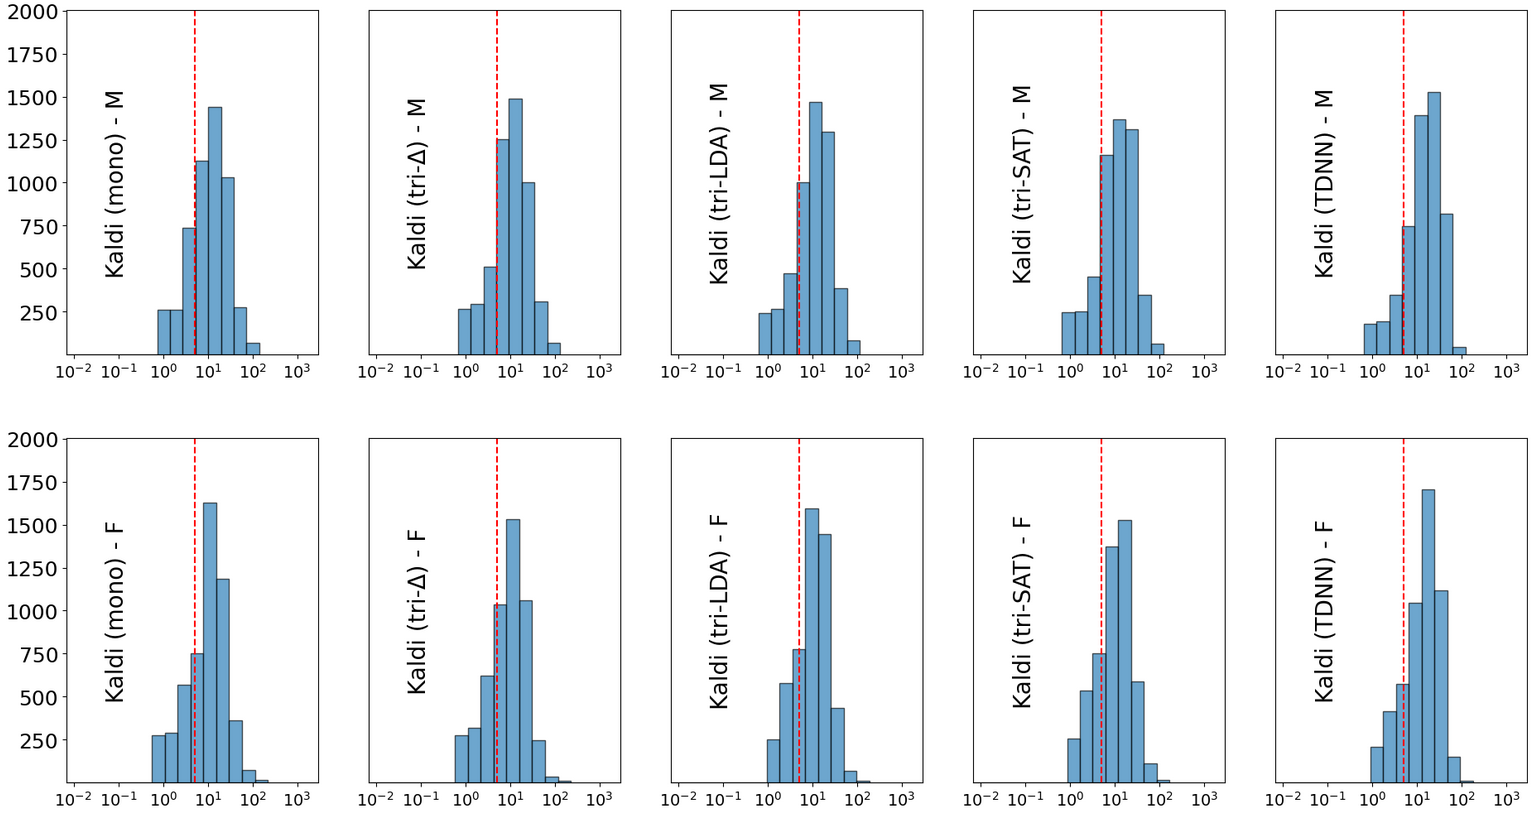
\includegraphics[width=\textwidth]{Figures/eurasip}
\end{center}
\caption{Histograma dos limites fon\'eticos entre o alinhamento for\c{c}ado e o alinhamento manual}
\end{figure}
\end{frame}

\begin{frame}
    \frametitle{Conclus�o}
    \begin{itemize}
        \item Os modelos ac�sticos treinados utilizando o Kaldi obtiveram resultados superiores � outros com suporte � l�ngua portuguesa, e t�o satisfat�rios quanto modelos para outras l�nguas
        \item Foi desenvolvido uma interface para utiliza��o do alinhador
        \item Fatores positivos:
            \begin{itemize}
                \item Avan�os na �rea de reconhecimento de voz para PT-BR
                \item Disponibiliza��o dos recursos desenvolvidos: \url{https://ufpafalabrasil.gitlab.io/}
            \end{itemize}
    \end{itemize}
\end{frame}

% \subsection{Trabalhos Futuros}
% % ----------------------------------------------------------------------------
% \begin{frame}{Trabalhos Futuros}
% \begin{itemize}
% % \item Expandir para outros sistemas operacionais: Windows, MacOS Android
% \item Solu��o alternativa ao \textit{headset}
% \item Sensores alternativos: Microfones de eletreto, BMP180 (press�o)
% \end{itemize}
% \end{frame}
%%% EOF %%%
